\documentclass[9pt,pdf,hyperref={unicode=true}]{beamer}
\usepackage[utf8]{inputenc}
\usepackage[russian]{babel}     %определение языков в документе
\usepackage{amssymb,amsmath}    %математика
\setbeamertemplate{frametitle}{
    \vspace{0.7cm}
    \insertframetitle
}
% Тема презентации
\usetheme{Boadilla}
%%%%%%%%%%%%%%%%%%%
%% Выбор шрифтов %%
\usefonttheme[onlylarge]{structurebold}

\usefonttheme{serif}
% Более крупный шрифт для подзаголовков титульного листа
\addtolength{\headsep}{1.6cm}

\setbeamerfont{institute}{size=\normalsize}
\setbeamersize{text margin left=10mm,text margin right=10mm}
%Отключение подписи Рис. у рисунков
\setbeamertemplate{caption}{\raggedright\insertcaption\par}

%%%%%%%%%%%%%%%%%%%
% Если используется последовательное появление пунктов списков на
% слайде (не злоупотребляйте в слайдах для защиты дипломной работы),
% чтобы еще непоявившиеся пункты были все-таки немножко видны.
\setbeamercovered{transparent}

%%%%%%%%%%%%%%%%%%
%%% Сокращения %%%
% Синий цвет выделения
\setbeamercolor{color1}{bg=blue!60!black,fg=white}
\newcommand{\celcius}{\,^{\circ}\mathrm{C}}  %градус Цельсия
\newcommand{\grad}{\,^{\circ}}               %знак градуса
\renewcommand{\epsilon}{\varepsilon}
%%%%%%%%%%%%%%%%%%
\newtheorem{theoremrus}{Теорема}
\title{Вычисление операторных экспонент}
\author{Автор: Алешин Дмитрий Алексеевич}
\date{2023}
\usepackage{multimedia}
\begin{document}

%%%%% 1 %%%%%

\begin{frame}
\begin{center}
{\fontsize{10pt}{12pt}\selectfont
ТВЕРСКОЙ ГОСУДАРСТВЕННЫЙ УНИВЕРСИТЕТ\\
МАТЕМАТИЧЕСКИЙ ФАКУЛЬТЕТ}\\
{\fontsize{10pt}{14pt}\selectfont
    Направление 02.03.01 Математика и Компьютерные науки\\
    Профиль «Математическое и компьютерное моделирование»} \\
\vspace{1.0cm}
{\fontsize{14pt}{14pt}\selectfont Алешин Дмитрий Алексеевич\\
\vspace{0.5cm}
\textcolor{blue!60!black}{ВЫЧИСЛЕНИЕ ОПЕРАТОРНЫХ \\
\vspace{0.3cm}
ЭКСПОНЕНТ В БАЗИСЕ ПАУЛИ}}\\
\vspace{0.5cm}
{\fontsize{10pt}{10pt}\selectfont
Научный руководитель: д. ф.-м. н. А. Н. Цирулёв}\\
\vspace{1.5cm}
{\fontsize{10pt}{10pt}\selectfont Тверь 2023}
\end{center}
\end{frame}

%%%%% 2 %%%%%

\begin{frame}[t]{Цели и задачи работы}
Цель работы --- изучить свойства операторной экспоненты для трехкубитных квантовых систем и разработать алгоритмы её вычисления с помощью разложения генерирующего оператора.
\vspace{0.5cm}

Задачи:
\begin{itemize}
\item{Изучить основные свойства базиса Паули}
\item{Рассмотреть возможные типы однородных трехкубитных гамильтонианов }
\item{Разработать алгоритм вычисления операторной экспоненты для трёх кубитов в базисе Паули}
\end{itemize}

\end{frame}

%%%%% 3 %%%%%

\begin{frame}[t]{Актуальность}

Теория квантовых вычислений продолжает быть актуальной на протяжении последних двух десятилетий.

Различные типы и подтипы квантовых вычислений адаптированы для различных технологий и аппаратных архитектур, но их математические структуры построены с использованием одних и тех же базовых понятий гильбертова пространства, квантовой наблюдаемости, унитарного оператора и квантового состояния.

\end{frame}

%%%%% 4 %%%%%

\begin{frame}[t]{Операторная экспонента и базис Паули}

Операторная экспонента используется в квантовой механике для описания эволюции квантовых систем во времени. Формула для вычисления операторной экспоненты через ряд Маклорена:
\begin{equation}
\text{e}^{\hat{A}}=\sum^{\infty}_{n=0}\frac{1}{n!} \hat{A}^n,
\end{equation}
где $\hat{A}$ - оператор, а $\hat{A}^n$ - его $n$-ая степень.

\vspace{0.3cm}

Базис Паули $P(\mathcal{H}_n)$ в $L(\mathcal{H}_n)$ (гильбертовом пространстве) определён как
\begin{equation} \label{eq1}
\{\hat{\sigma}_{k_1\ldots k_n}\}_{k_1,\ldots,k_n\in\{0,1,2,3\}},\quad \hat{\sigma}_{k_1\ldots k_n}=\hat{\sigma}_{k_1}\otimes \ldots \otimes \hat{\sigma}_{k_n},
\end{equation}
где $\hat{\sigma}_{0 \ldots 0}$ --- тождественный оператор. $P(\mathcal{H}_n)$ состоит из $4^n$ элементов.

В  \eqref{eq1} $k_1\ldots k_n$ --- строка Паули, $k_1, \ldots,  k_n \in \{0,1,2,3\}$. Для строк Паули мы будем использовать сокращённую запись $\hat{\sigma}_K$ = $\hat{\sigma}_{k_1,\ldots, k_n \in \{0,1,2,3\}}$, где $K$ --- десятичное представление числа $k_1\ldots k_n$, заданного в системе счисления по основанию 4.

\end{frame}

%%%%% 5 %%%%%

\begin{frame}[t]{Матрицы и операторы Паули}
Пусть $\{|0\rangle, |1\rangle \}$ являются ортонормированным базисом в некотором однокубитном пространстве в $\mathcal{H}$. Единичная матрица и матрицы Паули

\begin{equation}
	\hat{\sigma}_0=\begin{pmatrix}1 & 0 \\ 0 & 1\end{pmatrix},\quad
	\hat{\sigma}_1=\begin{pmatrix}0 & 1 \\ 1 & 0\end{pmatrix},\quad
	\hat{\sigma}_2=\begin{pmatrix}0 & -i \\ i & 0\end{pmatrix},\quad
	\hat{\sigma}_3=\begin{pmatrix}1 & 0 \\ 0 & -1\end{pmatrix},
\end{equation}
определим четыре оператора Паули
\begin{equation}
	\begin{array}{cc}
		\hat{\sigma}_0 = |0\rangle\langle0| + |1\rangle\langle1|, \quad \hat{\sigma}_1 = |0\rangle\langle1| + |1\rangle\langle0|,\\\\
		\hat{\sigma}_2 = -i|0\rangle\langle1| + i|1\rangle\langle0|, \quad \hat{\sigma}_3 = |0\rangle\langle0| - |1\rangle\langle1|,
	\end{array}
\end{equation}
которые эрмитовы и унитарны одновременно.
\end{frame}

%%%%% 6 %%%%%

\begin{frame}[t]{Общий вид гамильтониана}

Общий вид гамильтониана выглядит следующим образом:

\begin{equation}
	\hat{H} = \sum_{i,j,k\in\{0,1,2,3\}} h_{ijk}\hat{\sigma}_{ijk}.
\end{equation}

Но мы будем рассматривать специальный случай, когда гамильтониан состоит из трёх слагаемых и выглядит следующим образом:
\begin{equation}
\hat{H} = a\hat{\sigma}_A + b\hat{\sigma}_B + c\hat{\sigma}_C,
\end{equation}
где $a, b, c$ --- некоторые коэффициенты, а $\hat{\sigma}_A, \hat{\sigma}_B, \hat{\sigma}_C$ --- операторы Паули.\\
\vspace{0.5cm}
Классификация гамильтонианов:
\begin{enumerate}
\item $[\hat{\sigma}_A, \hat{\sigma}_B] = [\hat{\sigma}_A, \hat{\sigma}_C] = [\hat{\sigma}_B, \hat{\sigma}_C] = 0$
\item $\{\hat{\sigma}_A, \hat{\sigma}_B\} = \{\hat{\sigma}_A, \hat{\sigma}_C\} = \{\hat{\sigma}_B, \hat{\sigma}_C\} = 0$
\item $\{\hat{\sigma}_A, \hat{\sigma}_B\} = 0,\quad [\hat{\sigma}_A, \hat{\sigma}_C] = [\hat{\sigma}_B, \hat{\sigma}_C] = [\hat{\sigma}_A + \hat{\sigma}_B, \hat{\sigma}_C] = 0$
\item $[\hat{\sigma}_A, \hat{\sigma}_B] = 0,\quad \{\hat{\sigma}_A, \hat{\sigma}_C\} = \{\hat{\sigma}_B, \hat{\sigma}_C\} = 0$
\end{enumerate}

\end{frame}


%%%%% 7 %%%%%

\begin{frame}[t]{Вычисление композиции двух операторов Паули}

Для вычисления композиции двух операторов Паули $\hat{\sigma}_K$ и $\hat{\sigma}_L$ используется формула:
\begin{equation} \label{eq6}
\hat{\sigma}_K\hat{\sigma}_L = \omega\hat{\sigma}_M,
\end{equation}
где $\hat{\sigma}_M$ --- искомый оператор композиции, $\omega$ --- это $i$ или $-i$, которая вычисляется по формуле:
\begin{equation} \label{eq7}
\omega = (i)^{p+m}(-1)^m,
\end{equation}
где $p$ - количество соответствий 1-2, 2-3, 3-1, а $m$ - количество соответствий 2-1, 2-3, 1-3.

\end{frame}

%%%%% 8 %%%%%

\begin{frame}[t]{Алгоритм вычисления композиции двух операторов Паули и степеней гамильтониана}

Для вычисления композиции двух операторов Паули был реализован класс $Calculation$, который содержит следующие методы:
\begin{itemize}
\item $PauliMatrices$ --- рассчитывает $\hat{\sigma}_M$, используя формулу \eqref{eq6};
\item $Operations$ --- вычисляет $\hat{\sigma}_{ijk}$;
\item $Factors$ --- рассчитывает $\omega$, используя формулу \eqref{eq7}.
\end{itemize}

Для вычисления степеней гамильтониана был реализован класс $Hamiltonian$, который состоит из методов:

\begin{itemize}
\item $CountingOperators$ --- рассчитывает композицию операторов после композиции;
\item $CalculateSecondDegreeOfHamiltonian$ --- вычисляет вторую степень гамильтониана по формуле
$$H^2 = \hat{\sigma}_0 + 2ab \hat{\sigma}_A \hat{\sigma}_B;$$
\item $CalculateThirdDegreeOfHamiltonian$ --- вычисляет третью степень гамильтониана по формуле
 $$H^3 = H + 2ab^2\hat{\sigma}_A + 2a^2b\hat{\sigma}_B + 2abc\hat{\sigma}_A\hat{\sigma}_B\hat{\sigma}_C.$$
\end{itemize}

\end{frame}

%%%%% 9 %%%%%

\begin{frame}[t]{Входные данные и демонстрация работы программы}
Входные данные для работы программы подразумевают коэффициенты операторов Паули
$$
a, \quad b, \quad c
$$
и индексы операторов Паули
$$
\hat{\sigma}_A, \quad \hat{\sigma}_B, \quad \hat{\sigma}_C.
$$
\begin{figure}[h]
	\centering
	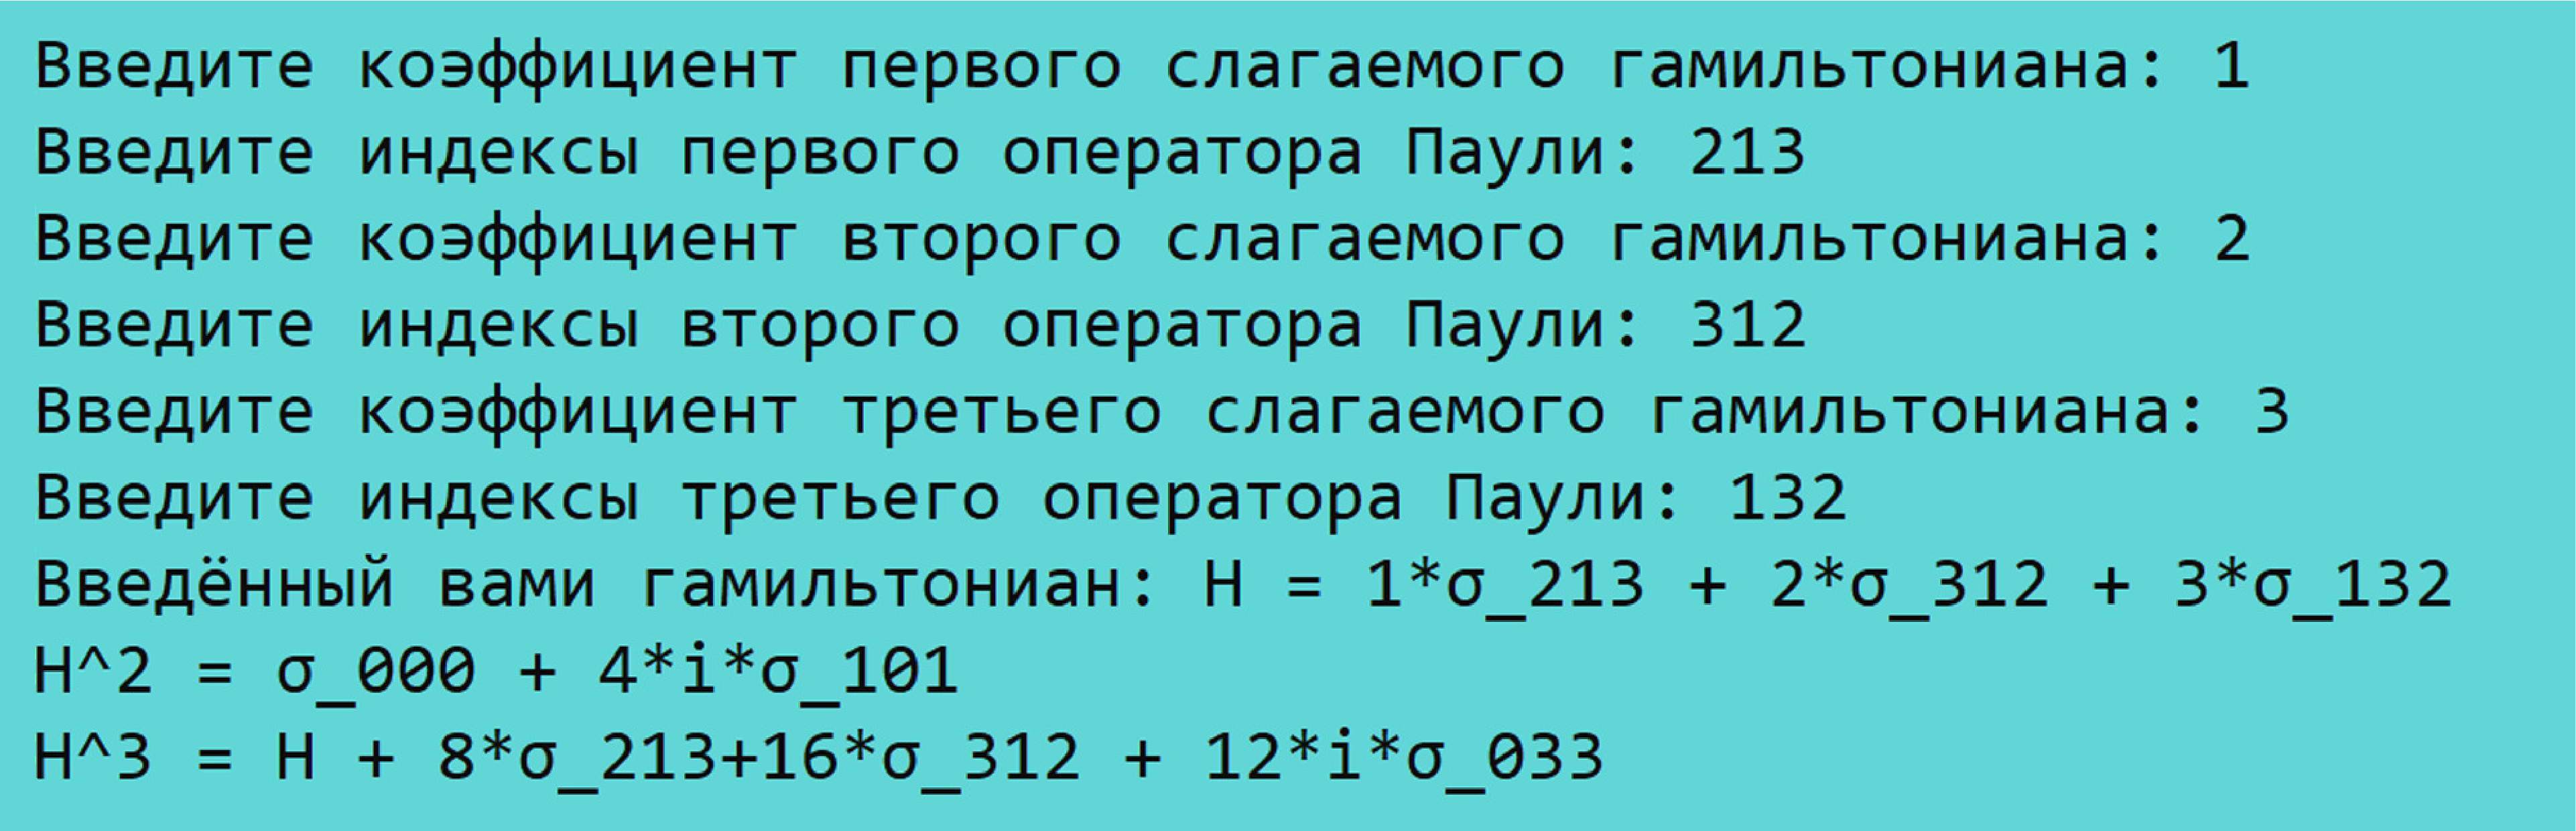
\includegraphics[width=1\linewidth]{screenshot_of_program_execution.pdf}
	\caption{Скриншот выполнения программы}
\end{figure}

\end{frame}

%%%%% 10 %%%%%

\begin{frame}[t]{Заключение}
В работе получены следующие основные результаты:
\vspace{0.4cm}
\begin{itemize}
\item{Изучены свойства базиса Паули}
\item{Рассмотрены возможные типы однородных трехкубитных гамильтонианов }
\item{Разработан алгоритм вычисления операторной экспоненты для трёх кубитов в базисе Паули на языке C$\#$}
\end{itemize}

\end{frame}

\end{document}




































